
\documentclass[11pt]{article}
%\usepackage{acl2012}
%\usepackage{color}
%\usepackage{times}
%\usepackage{url}
%\usepackage{latexsym}
\usepackage{booktabs}
\usepackage{graphicx}
\usepackage[noend]{algorithmic}
\usepackage{algorithm}
\usepackage{rotating}
\usepackage{verbatim}
\usepackage{amsmath}
%\usepackage{multirow}
%\usepackage{devanagari}

\newtheorem{sentence}{Sentence}


\title{REMOTELY ACCESING DOMESTIC SYSTEM  USING DTMF}

\author{
 173050046\\
 Department of Computer Science and Engineering\\
 Indian Institute of Technology Bombay\\
 {\small \tt  {173050046}@cse.iitb.ac.in} }



\begin{document}

\maketitle

\begin{abstract}
Wastage of Electricity (\textbf{\textit{one of the concerned topic now days}}) is increasing in proportional to its importance. The human mind always needs information of interest to control systems of his/her choice. In the age of electronic systems it is important to be able to control and acquire information from everywhere. Although many methods to remotely control systems have been devised, the methods have the problems such as the need for special devices and software to control the system. This model suggests a method for control using the\textbf{ DTMF }tone generated when the user pushes mobile phone keypad buttons or when connected to a remote mobile system. This allows user to remotely access various electric systems \textit{(lights, fans, motor ,etc.)}. The proposed work has been done experimentally and has been verified in real time. 
\end{abstract}


\section{Introduction}
The remote control technologies have been used in the fields like factory automation, space exploration, in places where human access is difficult. Controlling the domestic system regardless of time and space is an important challenge. As the mobile phone enables us to connect with the outside devices via mobile communication network regardless of time and space, the mobile phone is a suitable device to control domestic systems.
This model proposes a method to control a domestic system using a mobile phone, irrespective of the phone model and mobile phone carrier. The system suggested consists of the mobile phone normally registered in communication service and another mobile phone that can receive a call from another phone. This paper proposes to solve the problems of existing methods of control that use simple voice call. Method proposed uses the \textbf{\underline{DTMF}} (\textbf{Dual Tone Multi Frequency}) generated when a keypad button of the mobile phone is pressed by the user. The mobile phone user controls the system by sending the \textbf{\underline{DTMF}} tone to the access point. Mobile communication network coverage is larger than that of LANs, thus user can take advantage of mobile phones to control the system.


\begin{figure}[h]
\begin{center}
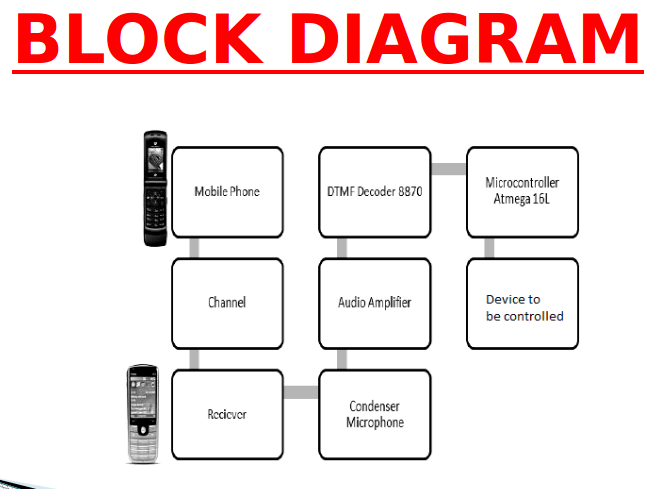
\includegraphics[scale=0.33]{blockdiag.png}
\caption{\label{fig:vaquois} Block diagram~\ref{fig:vaquois}}
\end{center}
\end{figure}

\section{Main components:}
\subsection{DTMF}
\begin{itemize}
\item{	DTMF (\textbf{Dual Tone Multiple Frequency)} is generic communication term for touch tone.
}
\end{itemize}
\begin{itemize}
	\item{
	The tone produced while dialling on the keypad of the phone could be used to represent the digits and a \textbf{separate tone} is used for each digit.
}
\end{itemize}
\begin{itemize}
	\item{
	Suggested that if two tones were used to represent a digit, the likelihood of a false signal occuring is ruled out.}
\end{itemize}
	
\section{Controller Circuit:}
	We have used \textbf{atmega-16 microcontroller}. It also uses relay switch to convert low signal to high signal. The reason behind using relay switch is, since our microcontroller works on \textbf{5 volt} and our home appliences works on \textbf{220} volts, so to convert a low signal into higher signal relay switch has been used. 

\begin{figure}[h]
	\begin{center}
		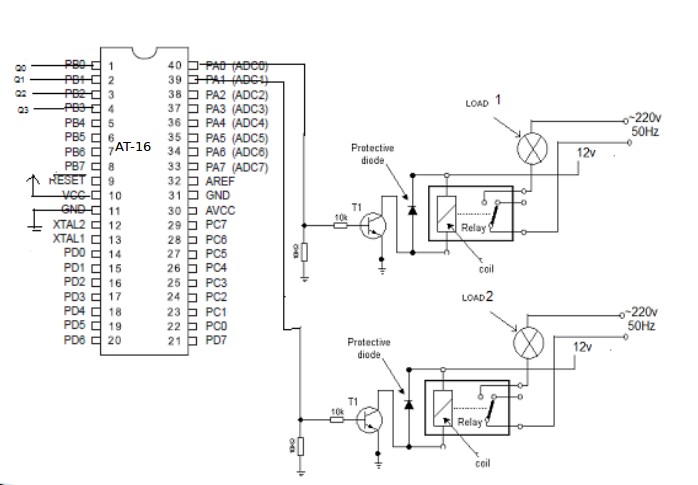
\includegraphics[scale=0.33]{circuit.png}
		\caption{\label{fig:vaquois} Circuit diagram}
	\end{center}
\end{figure}

\section{Programming :}
	In this project we have used C programming language to program our \underline{Atmega-16} microcorntroller. Programme is transferred through \textbf{\underline{USB tiny}}. We used Eclipse framework to write and execute our program.


\begin{figure}[h]
	\begin{center}
		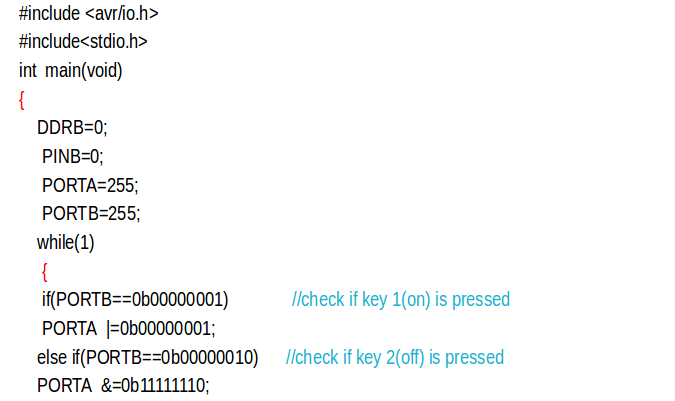
\includegraphics[scale=0.33]{program.png}
		
	\end{center}
\end{figure}

\section{Application :}
Followings are some other application of this system.
\begin{itemize}
	\item{Combinational Lock}
\end{itemize}
\begin{itemize}
	\item{Home Secuity System}
\end{itemize}
\begin{itemize}
	\item{Mobile/Wireless Robot control}
\end{itemize}
\begin{itemize}
	\item{Wireless Radio Control}
\end{itemize}
\begin{itemize}
	\item{Continuous monitoring of system status}
\end{itemize}
\begin{itemize}
	\item{Remote Switches}
\end{itemize}

\section{Conclusion :}
This system presents a method to control domestic appliences. It uses commercial mobile communication network as a path of data transmission. It also reduces wastage of electrical power to a large extent. This is a very low cost operation system. The feedback from the receiving circuit is not possible but can be solved by using \textbf{GSM} module.

\section{Mathematical Equations:}
\begin{itemize}
\item
The binomial coefficient is defined by the next expression:
\end{itemize}
$$
\binom{n}{r} = \frac{n!}{r!(n-r)!}
$$
\begin{itemize}
\item
Differentiation of an integreal of a function is function itself.
\end{itemize}
 $$
 \frac{d}{dx}\left( \int_{0}^{x} f(u)\,du\right)=f(x).
 $$


\section{Bar-Chart:}
Data of this bar chart is taken from a csv file.
 

\begin{figure}[h]
	\begin{center}
		\includegraphics[scale=0.33]{image2.pdf}
		
	\end{center}
\end{figure}

\section{Line-Graph :}
I have used some hard-coded data for this line graph. 
This graph shows relationship between \textbf{\textit{side }}of a square and its \textbf{\textit{area}}.
 

\begin{figure}[h]
	\begin{center}
		\includegraphics[scale=0.33]{image1.pdf}
		
	\end{center}
\end{figure}

\section{Histogram :}
This is Gaussian histogram where data is generated randomly. The data is randomly distributed between 0 and 1000.\textbf{\textit{X-axis}} of this histogram represents the random value and \textbf{\textit{Y-axis}} represents the frequency of the random value.
 

\begin{figure}[h]
	\begin{center}
		\includegraphics[scale=0.33]{image3.pdf}
		
	\end{center}
\end{figure}



\section{Red circled point graph :}
This is a red circled point graph where input data is hard coded. Input data is random here and so is graph.
 

\begin{figure}[h]
	\begin{center}
		\includegraphics[scale=0.33]{image4.pdf}
		
	\end{center}
\end{figure}
\section{Table : }
This table contains random data between 0 and 1 of size 4*5 matrix.\\

\input{table}

\end{document}









